\section{Auswertung}

\subsection{Vorbereitung}

Zur Vorbereitung für diesen Versuch wird die Schallgeschwindigkeit $c$ und die
akustische Impedanz $Z$ von einigen Materialien bestimmt. Sie sind in Tabelle \ref{tab:1}
gezeigt.

\begin{table}[H]
  \centering
  \caption{Literaturwerte für Schallgeschwindigkeiten und akustischen Impedanzen \cite{2}.}
  \label{tab:1}
  \begin{tabular}{c c c}
    \toprule
     & $c \, / \, \si[per-mode=fraction]{\meter\per\second}$ & $Z \, / \, \si[per-mode=fraction]{\kilo\gram\second\per\meter\tothe{4}}$ \\
     \midrule
     Luft \SI{0}{\celsius}          & 331  & \num{427e3}  \\
     dest. Wasser \SI{20}{\celsius} & 1485 & \num{1483e3} \\
     Blut                           & 1560 & \num{1.6e6} \\
     Acryl                          & 2730 & \num{3.22e6} \\
     \bottomrule
  \end{tabular}
\end{table}

Als erstes wird von einem Acrylzylinder, mit dem Puls-Echo-Verfahren, die Schallgeschwindigkeit
bestimmt. Dazu ist die Höhe des Zylinders, mit den zugehörigen Messergebnissen in
Tabelle \ref{tab:2} abgebildet. Für die Schallgeschwindigkeit wird die Formel \ref{eq:6} verwendet.

\begin{table}[H]
  \centering
  \caption{Abmessungen und Messergebnisse des ersten Acrylzylinders.}
  \label{tab:2}
  \begin{tabular}{c c c c c c c}
    \toprule
    & \multicolumn{2}{c}{Puls 1} & \multicolumn{2}{c}{Puls 2} \\
    \cmidrule(lr){2-3}\cmidrule(lr){4-5}
    $L\, / \, \si{\centi\meter}$ & $U\, / \,  \si{\volt}$ & $t \, / \,  \si{\micro\second}$ &
    $U\, / \,  \si{\volt}$ & $t \, / \,  \si{\micro\second}$ & $\Delta t \, / \,  \si{\micro\second}$ &
    $c \, / \,  \si[per-mode=fraction]{\meter\per\second}$ \\
    \midrule
    3,935 & 1 & 30,1 & 0,118 & 59 & 28,9 & 2723,18 \\
    \bottomrule
  \end{tabular}
\end{table}

\begin{figure}[H]
  \centering
  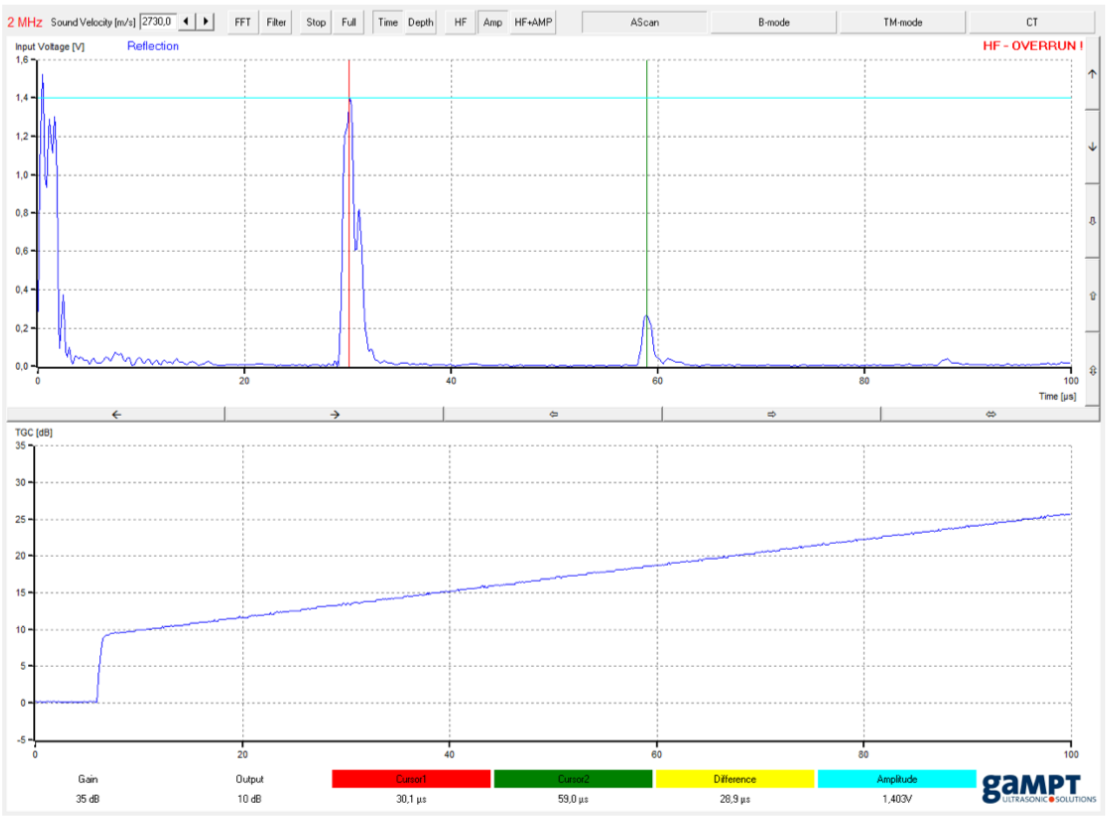
\includegraphics{content/Programm.png}
  \caption{Darstellung des Messprogramms für den ersten Zylinder.}
  \label{abb:1}
\end{figure}

In der Abbildung \ref{abb:1} ist das Messprogramm dargestellt. Zur Bestimmung der
Schallgeschwindigkeit in dem Acrylzylinder werden die Pulse verwendet, die durch
den roten und blauen Cursor markiert sind. Die Amplituden werden auch an diesen Stellen
bestimmt.

Nun wird die bestimmte Schallgeschindigkeit von $c = \SI{2723.18}{\meter\per\second}$
in das Messprogramm eingetragen und es wird eine Tiefenmessung durchgeführt.
Diese ergibt:

\begin{equation*}
  L = \SI{3.92}{\centi\meter}.
\end{equation*}

Das ist eine Abweichung von $0,38 \%$.

\subsection{Bestimmung der Dämpfung}

Nun wird die Dämpfung bestimmt. Die Messwerte sind in Tabelle \ref{tab:3} dargestellt.

\begin{table}[H]
  \centering
  \caption{Messwerte der Amplituden von verschiedenen Acrylzylindern.}
  \label{tab:3}
  \begin{tabular}{c c c}
    \toprule
    1. Amplitude / V & 2. Amplitude / V & Länge / cm \\
    \midrule
    1,538 & 1,040 &  8,020 \\
    1,538 & 0,418 & 10,250 \\
    1,538 & 1,150 &  6,130 \\
    1,538 & 0,338 & 12,025 \\
    1,538 & 1,361 &  3,100 \\
    1,538 & 1,346 &  3,935 \\
    \bottomrule
  \end{tabular}
\end{table}

Dazu wird die Gleichung \ref{eq:4} umgeformt zu:

\begin{equation*}
 \ln(\frac{I(x)}{I_0}) = - \alpha x.
\end{equation*}

Nun lässt sich mit dueser Formel eine lineare Ausgleichsrechnung durchführen.
In Abbildung \ref{abb:2} sind die Messerte und die Ausgleichsrechnung gezeigt.

\begin{figure}[H]
  \centering
  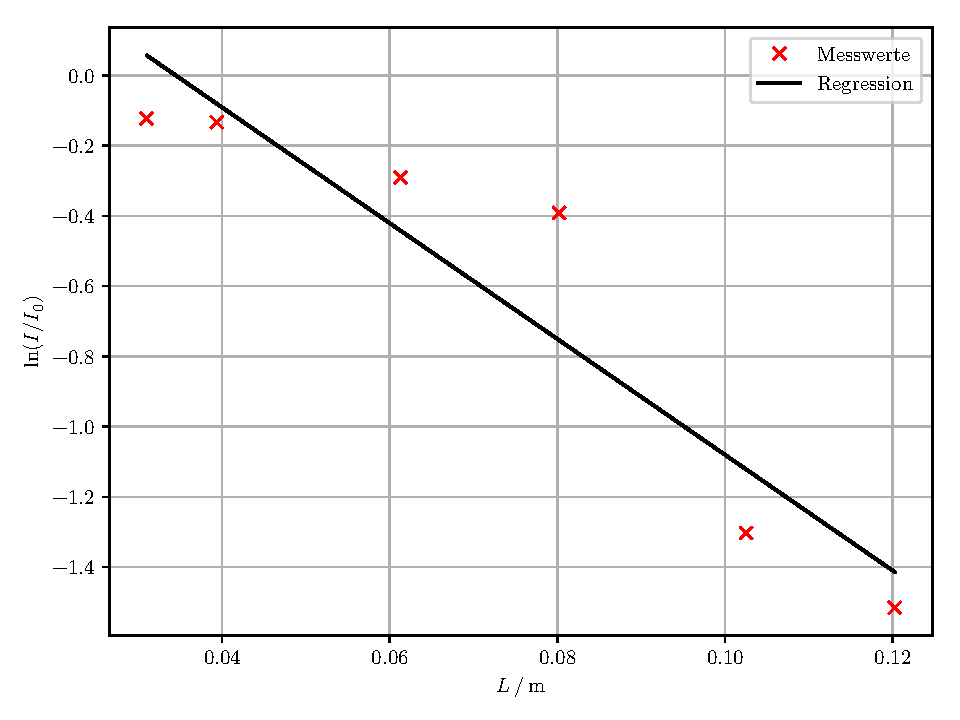
\includegraphics{plot1.pdf}
  \caption{Messwerte und lineare Ausgleichsrechnung der Dämpfung.}
  \label{abb:2}
\end{figure}

Die Ausgleichsrechnung wird mit Python 3.6 durchgeführt. Es ergibt sich für die Parameter
der Geraden:

\begin{itemize}
  \item $\alpha = \SI{16.48(307)}{\per\meter}$
  \item $b = \num{0.57(24)}$
\end{itemize}

Dabei ist b der Achsenabschnitt.

\subsection{Schallgeschwindigkeit Impuls-Echo-Verfahren}

In diesen Abschnitt wird die Schallgeschwindigkeit von verschiedenen Acrylzylindern
bestimmt. Dabei werden zunächst die Zylinder vermessen und daraufhin wird die Laufzeit
gemessen. Mit der Gleichung \ref{eq:6} kann aus den Werten die Schallgeschwindigkeit
bestimmt werden. Die Messwerte sind in Tabelle \ref{tab:4} dargestellt.

\begin{table}[H]
  \centering
  \caption{Darstellung der Laufzeiten und Schallgeschwindigkeiten verschiedener
  Acrylzylinder.}
  \label{tab:4}
  \begin{tabular}{c c c}
    \toprule
    $L \, / \, cm$ & $\Delta t \, / \, \si{\micro\second}$ & $c \, / \, \si{\meter\per\second}$ \\
    \midrule
     3,100 & 23,0 & 2695,65 \\
     3,935 & 28,9 & 2723,18 \\
     6,130 & 45,5 & 2694,51 \\
     8,020 & 59,2 & 2709,46 \\
    10,250 & 75,9 & 2700,92 \\
    11,955 & 87,9 & 2720,14 \\
    12,025 & 88,3 & 2723,67 \\
    \bottomrule
  \end{tabular}
\end{table}

Keine Ahnung

\subsection{Schallgeschindigkeit Durchschallungs-Verfahren}

Als nächstes wird mit dem Durchschallungs-Verfahren die Schallgeschwindigkeit
der Acrylzylinder bestimmt. Dabei wird wieder mit der Gleichung \ref{eq:6} die
Schallgeschindigkeit bestimmt, es ist diesmal nur nicht nötig die Laufzeit zu halbieren,
da die der Ultraschall den Zylinder nur einmal durchläuft. Die Messwerte sind in
Tabelle \ref{tab:5} dargestellt.

\begin{table}[H]
  \centering
  \caption{Laufzeiten und Schallgeschindigkeiten bei dem Durchschallungs-Verfahren.}
  \label{tab:5}
  \begin{tabular}{c c c}
    \toprule
    $L \, / \, cm$ & $\Delta t \, / \, \si{\micro\second}$ & $c \, / \, \si{\meter\per\second}$ \\
    \midrule
     3,100 & 11,55 & 2683,98 \\
     3,935 & 14,85 & 2649,83 \\
     6,130 & 22,75 & 2694,51 \\
     8,020 & 29,50 & 2718,64 \\
    10,250 & 38,80 & 2641,75 \\
    12,025 & 45,00 & 2672,22 \\
    \bottomrule
  \end{tabular}
\end{table}
